\subsection{Variaci\'on de la resistencia $R_8$}

\todo{HACER}

\subsection{Variaci\'on de la resistencia $R_6$}

A continuaci\'on se muestra c\'omo cambian los polos y ceros al modificar la resistencia R6 en la expresi\'on de la transferencia \ref{vovi}, dejando fijas las otras resistencias y los capacitores con los valores determinados para hacer el filtro.


\begin{figure}[H] %!ht
	\centering
	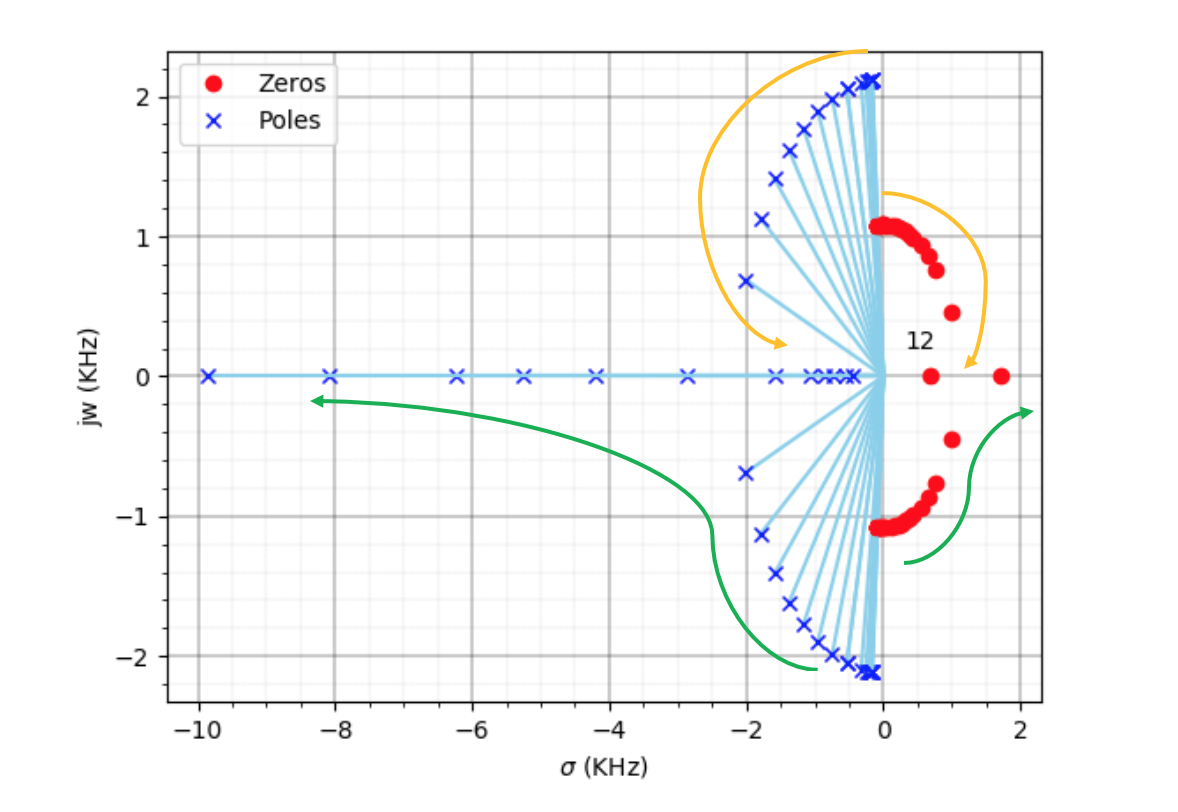
\includegraphics[width=10cm,height=10cm,keepaspectratio]{../EJ1/00GRAFICOS/r6.png}
	\caption{Polos y ceros del circuito al tender R6 a cero}
	\label{r6}
\end{figure}

En la figura \ref{r6} se indica con flechas hacia donde tienden los polos y los ceros al hacer tender R6 a cero. Las flechas amarillas corresponden a la variaci\'on del polo $P1$ y del cero $Z1$ en dicho caso, mientras que las flechas verdes indican el comportamiento del polo $P2$ y del cero $Z2$. Para el caso en el que R6 tiende a infinito, las flechas van en sentido contrario al indicado en la figura. A continuaci\'on se muestran anal\'iticamente dichos comportamientos:

\begin{equation}
	\lim_{R_6\to 0} s_{z1,z2}=  \frac{R_4 R_5}{C_6 R_6 R_8} \pm \frac{R_4 R_5}{C_6 R_6 R_8} \Rightarrow 
	\begin{cases} 
	s_{z1} \to +\infty\\
	s_{z2} \to 0
	\end{cases}
\end{equation}

\begin{equation}
	\lim_{R_6\to 0} s_{p1,p2}=  -\frac{R_6 + R_7}{C_6 R_6 R_7} \pm \frac{R_6 + R_7}{C_6 R_6 R_7} \Rightarrow
	\begin{cases} 
	s_{p1} \to 0\\
	s_{p2} \to -\infty
	\end{cases}
\end{equation}

\begin{equation}
\lim_{R_6\to\infty}s_{z1,z2} =  
\end{equation}

\begin{equation}
\lim_{R_6\to\infty}s_{p1,p2} =  
\end{equation}

